\documentclass{article}
    
\usepackage{Haust2017skil}

\title{Stærðfræðimynstur í tölvunarfræði \\ Skilaverkefni 8}
\author{}

\begin{document}
\maketitle

Skila skal þessu verkefni á vefnum \href{https://gradescope.com/courses/9487}{Gradescope}. Aðgangskóði fyrir námskeiðið er \textbf{9N834D}. 

Gradescope tekur við .pdf skjölum. Frágangur á þeim skiptir máli. Þau skulu vera hreinskrifuð í tölvu. Kerfi eins og \LaTeX, Google Docs og Microsoft Word geta búið til .pdf skjöl. Mikilvægt er að merkja á hvaða blaðsíðu .pdf skjalsins hver lausn kemur fyrir, ekki er hægt að gera ráð fyrir að dæmatímakennarar fari yfir ómerkt dæmi.

Skila má þessum dæmum sem einstaklingar eða \emph{tvö og tvö saman}.

Telji nemandi að mistök hafi verið gerð við yfirferð skal tilkynna slíkt með tölvupósti til dæmatímakennara. Nálgast má lista yfir hvaða dæmatímakennari fór yfir hvaða dæmi á Piazza-vef námskeiðsins.

\section{Kafli 9.1}

\question

\paragraph{(Ísl):} Útskýrið hvort eftirfarandi vensl $R$ á mengi alls fólks séu sjálfhverf, samhverf, andsamhverf og/eða gegnvirk, þar sem $(a,b)\in R$ þá og því aðeins að
\begin{enumerate}[a)]
    \item $a$ er hærri en $b$
    \item $a$ og $b$ eiga sama afmælisdag
    \item $a$ og $b$ hafa sama nafn
    \item $a$ og $b$ eiga sömu ömmu
\end{enumerate}

\paragraph{(En):} Determine whether the relation $R$ on the set of all people
is reflexive, symmetric, antisymmetric, and/or transitive,
where $(a,b)\in R$  if and only if

\begin{enumerate}[a)]
    \item $a$ is taller than $b$.
    \item $a$ and $b$ were born on the same day.
    \item $a$ has the same first name as $b$.
    \item $a$ and $b$ have a common grandparent.
\end{enumerate}

\paragraph{Í bók:} 9.1.4 í International/Icelandic, ekki til staðar í Global

\question Sýnið að tómu venslin $R=\emptyset$ á mengi sem ekki er tómt séu samhverf og gegnvirk en ekki sjálfhverf.

\paragraph{Í bók:} 9.1.8 í International/Icelandic, 9.1.6 í Global

\section{Kafli 9.3}

\question Útskýrið hversu mörg stök í í fylkinu sem táknar venslin á mengið $A=\{1,2,\ldots,1000\}$ sé $R$\ldots

\begin{enumerate}[a)]
    \item $\{(a,b)| a \leq b\}$
    \item $\{(a,b)| a = b\pm 1$
    \item $\{(a,b)| a+b=1000\}$
\end{enumerate}

\paragraph{Í bók:} Hluti af 9.3.10 í Icelandic/International, 9.3.6 í Global

\question

\paragraph{(Ísl):}
\begin{enumerate}[a)]
    \item Teiknið stefnt net fyrir venslin $\{(a, a), (a, b), (b, c), (c, b), (c, d), (d, a), (d, b)\}$.
    \item Teljið upp röðuðu pörin í venslunum sem netið að neðan skilgreinir:
\end{enumerate}

\paragraph{(En):}
\begin{enumerate}[a)]
    \item  Draw the directed graph that represents the relation
    $\{(a, a), (a, b), (b, c), (c, b), (c, d), (d, a), (d, b)\}$.
    \item List the ordered pairs in the relation represented by the following digraph:
\end{enumerate}

\begin{center}
 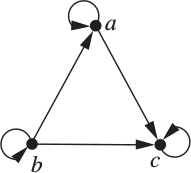
\includegraphics[width=0.33\textwidth]{triangle-graph}
\end{center}
\paragraph{Í bók:} 9.3.22 og 9.3.24 í International/Icelandic, ekki til staðar í Global

\section{Kafli 9.2}

\question Gefin er eftirfarandi tafla:
\begin{center}
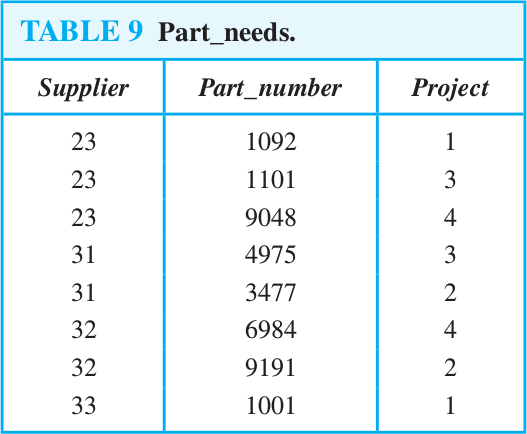
\includegraphics[width=0.6\textwidth]{parts-table}
\end{center}
ásamt eftirfarandi SQL-skipun sem vinnur á töflunni:
\begin{minted}[frame=lines]{sql}
SELECT Supplier
FROM Part_needs
WHERE 1000 <= Part_number AND Part_number <= 5000
\end{minted}
Svo er spurt:

\begin{enumerate}[a)]
 \item Hvaða aðgerðir (venslavirkjar) koma við sögu í þessari SQL-skipun og hvaða áhrif hefur hver þeirra á niðurstöðuna?
 \item Hver er niðurstaða þessarar SQL-skipunar?
\end{enumerate}

\paragraph{Í bók:} Exercise 9.2.28

\question

\paragraph{(Ísl):} Skrifið SQL-skipun sem sýnir í hvaða herbergi Rosen prófessor er að kenna klukkan 3 síðdegis.

Sjá gagnagrunnsuppsetningu á \href{http://sqlfiddle.com/#!9/14848/1}{SQL Fiddle}.

\paragraph{(En):} Write an SQL-statement that shows in which room professor Rosen is teaching at 3 PM.

See the database set up at \href{http://sqlfiddle.com/#!9/14848/1}{SQL Fiddle}.

\paragraph{Í bók:} Dæmið er ekki í bókinni.

\end{document}
